
\documentclass[a4paper, 12pt]{article}
\usepackage{geometry}
\geometry{margin=2cm}
\usepackage{graphicx} % Required for the inclusion of images
\usepackage[utf8]{inputenc}
%\usepackage{natbib} % Required to change bibliography style to APA
\usepackage{amsmath} % Required for some math elements 
\usepackage[spanish]{babel} 
%\usepackage{fontspec}
\usepackage{lineno,hyperref}
\usepackage{upgreek}
\usepackage{gensymb}
\usepackage{textcomp}
\usepackage{amssymb}
\usepackage{textgreek}
\usepackage{float}
\usepackage{fancyhdr}
\usepackage{dirtytalk}

\allowdisplaybreaks
%\textwidth18cm
%\textheight22cm
%\topmargin0cm
%\oddsidemargin2cm
%\hypersetup{hidelinks}

\usepackage{multirow}

\hypersetup{
    colorlinks=true,
    linkcolor=blue,
    }
\graphicspath{{img}}
\setlength\parindent{0pt} % Removes all indentation from paragraphs

\renewcommand{\labelenumi}{\alph{enumi}.} % Make numbering in the enumerate environment by letter rather than number (e.g. section 6)

\renewcommand{\b}{\textbf}

\newsavebox{\mygraphic}
\sbox{\mygraphic}{
\includegraphics[height=1cm]{logoUNRN.jpg}}


\pagestyle{fancy}

\fancyhead{}

\headheight 16pt

\fancyhead[LO]{\setlength{\unitlength}{1in}
	\begin{picture}(0,0)
		\put(0,0){\usebox{\mygraphic}}
	\end{picture}
	\hspace{1cm}
}

\fancyhead[CO] {\hspace{1.5cm} \large Física I: Ingenierías Ambiental, Electrónica y Telecomunicaciones}

%esto me pareció piola para enumerar los ejercicios
%lo saqué de acá: https://tex.stackexchange.com/questions/302948/numbered-exercises-as-sections
%%%%%%%%%%%%%%%%%%%%%%%%%%%%%%%%%%%%%%%%%5
\newcounter{eje}
\setcounter{eje}{0}
\newcounter{subeje}
\setcounter{subeje}{-1}
\renewcommand\thesubeje{\arabic{eje}\alph{subeje}}%
\newcommand \eje{%
  \vspace{.2cm}
  \par\noindent
  \ifnum\value{subeje}>-1
    \refstepcounter{subeje}%
    \llap{\thesubeje)\quad}%
  \else
    \refstepcounter{eje}%
    \llap{\theeje)\quad}%
  \fi
}
\begin{document}
\pagestyle{fancy}

\begin{center}

	{\Large \textbf{Primer parcial}}
 
\vspace{.2cm}

{viernes 8/9}
\end{center}

Tome para el valor de g = 9.8 m/s$^2$.

\eje{\bf TEMA 1: CINEMÁTICA} Una persona lanza un palito a 30 km/hr con un ángulo de 45$\degree$ respecto de la horizontal (el suelo). Simuláneamente, un perro galgo, que se encontraba a su lado, corre a buscar el palito partiendo desde el reposo, pero acelerando de manera constante hasta que lo atrapa.
Encuentre:

a) el valor de la aceleración del galgo, y 

b) la velocidad del canino cuando toma el palito. 

Suponga para ello, que la altura a la que la mano de la persona se desprende del palito y la altura a la que el perro lo atrapa, son la misma.


\eje{\bf TEMA 2: DINÁMICA DE UNA PARTÍCULA} Dos cajas están conectadas por una polea como se muestra en el dibujo. La caja 'A' tiene una masa m$_A$ = 2 kg, mientras que la caja 'B' tiene masa m$_B$ = 3 kg y, el coeficiente de roce estático entre ambas cajas, es de 0.5. Además, considere que entre la caja 'B' y la mesa no hay rozamiento. Entonces:

a) ¿cuál es la fuerza \b F máxima que puede ejercerse sobre la caja de arriba ('A') sin que deslicen entre sí? 

\begin{figure}[H]
\begin{center}
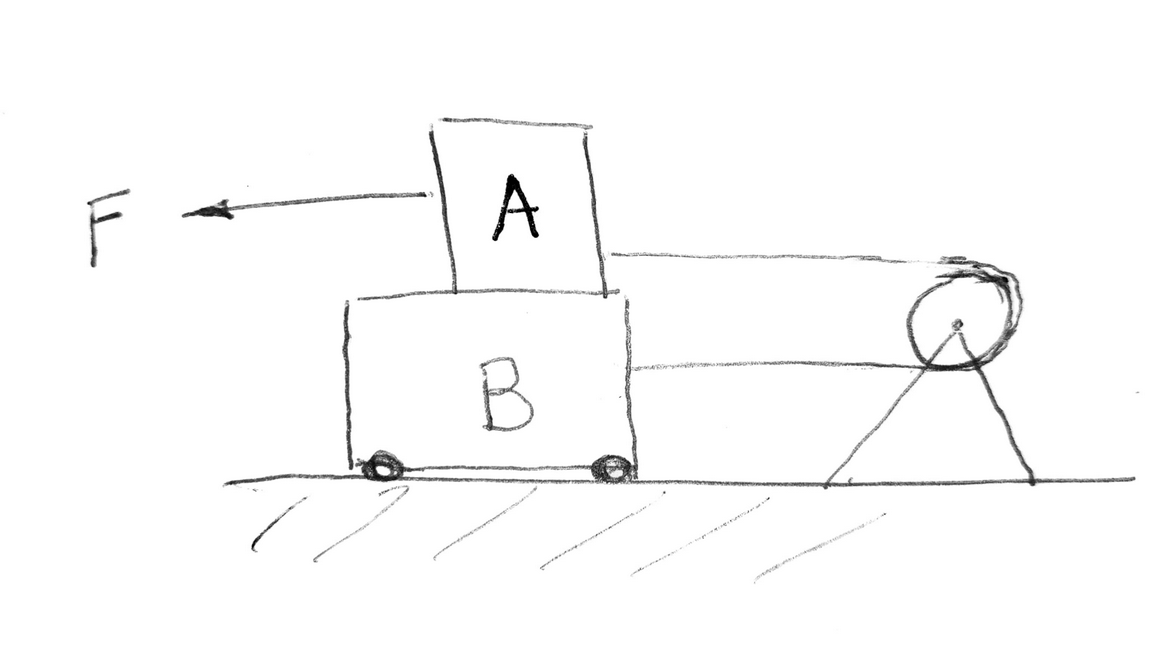
\includegraphics[clip,width = .45\columnwidth]{img/1erparcial2023-0.png}
\end{center}
\end{figure}

\end{document}